\documentclass[micros_g1_main.tex]{subfiles}
\begin{document}

\section{Ejercicio 3}
A continuación se presenta una foto del microcontrolador corriendo el programa Blink con el LED correspondiente en verde con una frecuencia de 0.5Hz, como requería la consigna.
	\begin{figure}[H]
		\centering
		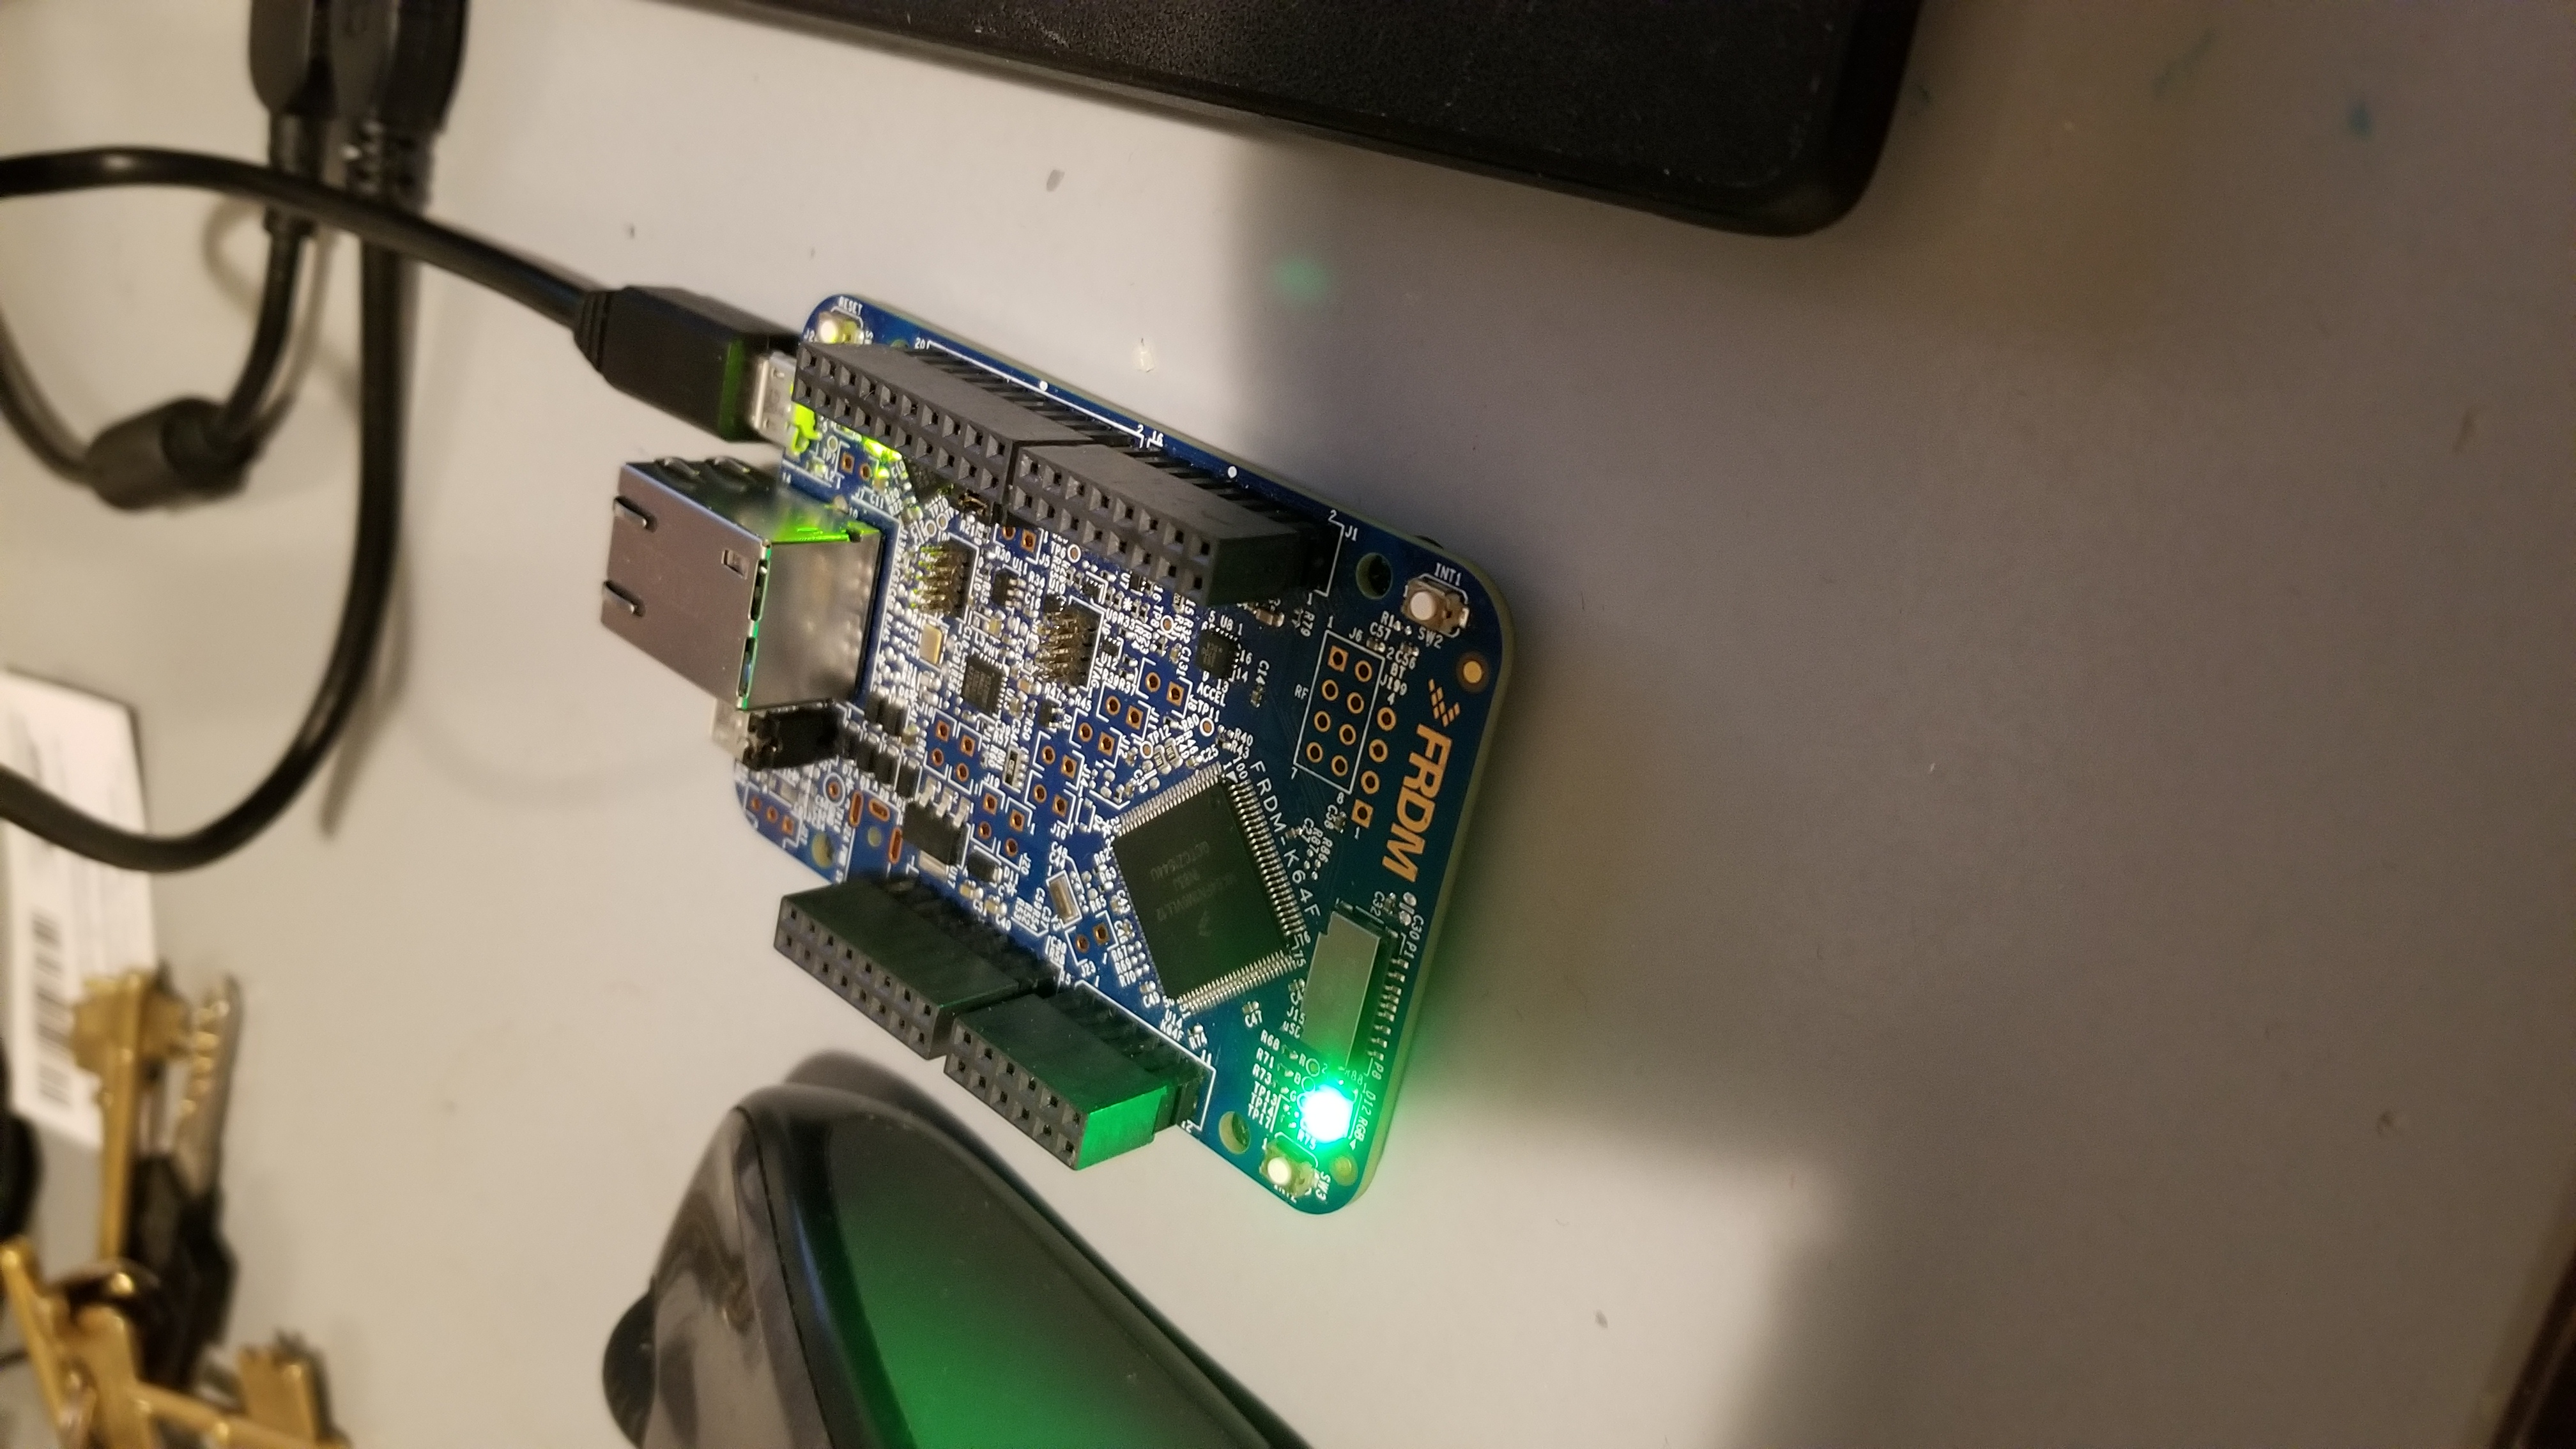
\includegraphics[width=0.45\textwidth]{images/blink_green.jpg}
		\caption{Corriendo el programa Blink} \label{fig:cct}
	\end{figure}

A fin de poner en evidencia la frecuencia a la que se produce el blink, se muestra a continuación una imagen del pin correspondiente:
	\begin{figure}[H]
		\centering
		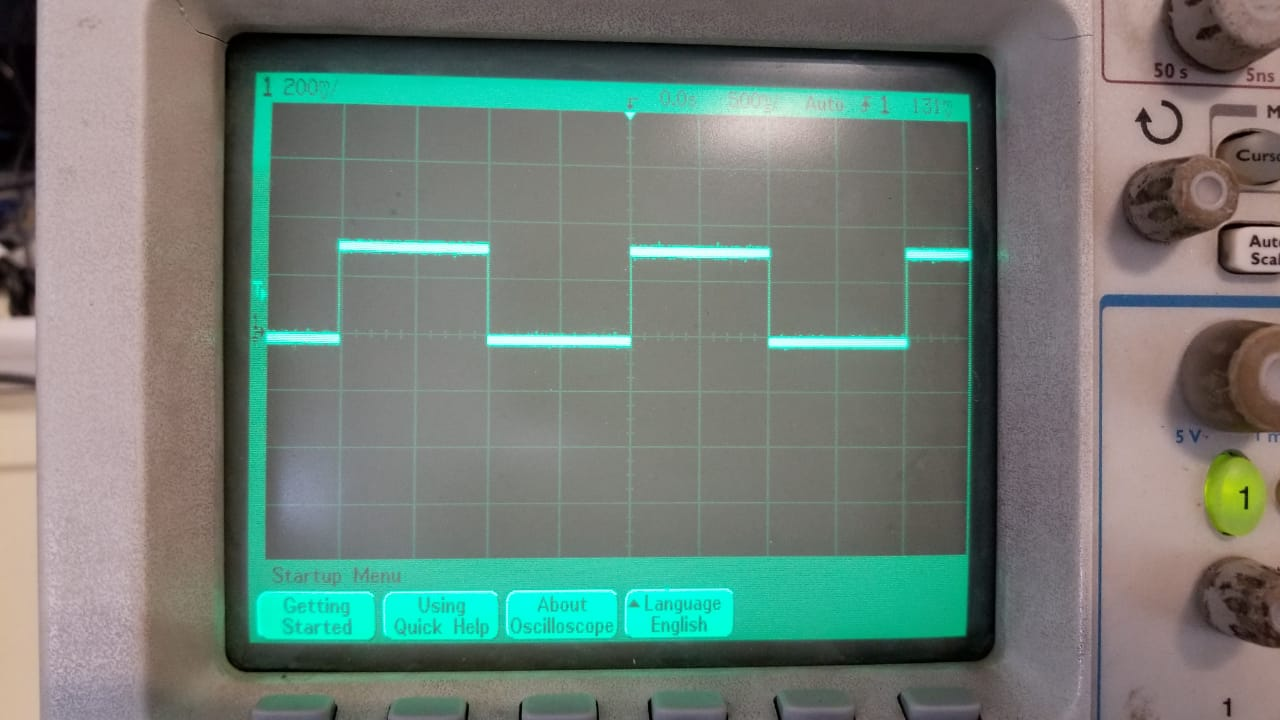
\includegraphics[width=0.45\textwidth]{images/blink_green_1s.jpeg}
		\caption{Corriendo el programa Blink con el LED en verde y a una frecuencia de 0.5Hz} \label{fig:cct}
	\end{figure}

\end{document}
